\documentclass[a4paper, 12pt]{article}
\NeedsTeXFormat{LaTeX2e}[1996/06/01]
\usepackage[usenames]{color} 
\usepackage{amsmath,amssymb}
\numberwithin{equation}{section}
\usepackage[top=2.5cm,left=3cm,right=3cm,bottom=3cm,foot=1cm,]{geometry}
%\linespread{1.5}
\usepackage[breaklinks, colorlinks, citecolor=blue]{hyperref}
\usepackage{multirow,array,graphicx}
\usepackage{sidecap,epstopdf,dcolumn}
\usepackage{bm}% bold math
\usepackage[font={small,it}]{caption}
\usepackage[footnotesize]{subfigure}
\usepackage[]{appendix}
%%%% Make citations use [1-5] rather than [1, 2, 3, 4, 5]
\usepackage[numbers, square, comma,  sort&compress]{natbib}
%\renewcommand{\cite}{\citep}
%%%% END
%\usepackage{ulem}
\setcounter{tocdepth}{3}
\setcounter{secnumdepth}{3}
\newcommand{\note}[1]{{\color{blue}[#1]}}


\renewcommand{\sectionmark}[1]{\markright{\thesection.\ #1}{}}


\newcommand{\Planck}{{\textit{Planck }}}
\newcommand{\SPT}{{\textit{SPT }}}
\newcommand{\CFHTLenS}{{\textit{CFHTLenS }}}
\newcommand{\CoRE}{{\textit{CoRE }}}
\newcommand{\WMAP}{{\textit{WMAP }}}
\newcommand{\Euclid}{{{\it Euclid}}}
\newcommand{\CAMB}{{\tt{CAMB }}}
\newcommand{\MGCAMB}{{\tt{MGCAMB }}}

%\newcommand{\vphi}[0]{{\color{green}{\delta\phi}}}
%\newcommand{\dlg}[0]{{\color{red}{\lp g}}}
\newcommand{\vphi}[0]{\delta\phi}
\newcommand{\lpa}[0]{\lp A}
\newcommand{\dlg}[0]{\lp g}

\newcommand{\depg}[0]{\ep g}
\newcommand{\virt}[0]{\hat{\delta}}
\newcommand{\Dvphi}[1]{\nabla_{#1}\vphi}
\newcommand{\DDvphi}[2]{\nabla_{#1}\nabla_{#2}\vphi}

\newcommand{\Dvvphi}[1]{\nabla_{#1}\virt\vphi}
\newcommand{\DDvvphi}[2]{\nabla_{#1}\nabla_{#2}\virt\vphi}

\newcommand{\tmat}[4]{\left( \begin{array}{cc} #1 & #2 \\ #3 & #4 \end{array}\right)}
\newcommand{\expec}[1]{\left\langle #1\right\rangle}
\newcommand{\half}[0]{\frac{1}{2}}
\newcommand{\cs}[3]{\Gamma^{#1}_{\,\,\,\, #2#3}}

\newcommand{\pd}[2]{\frac{\partial #1}{\partial #2}}
\newcommand{\ld}[0]{\mathcal{L}}
\newcommand{\md}[0]{\mathcal{M}}
\newcommand{\dd}[0]{\textrm{d}}
\newcommand{\defn}[0]{\equiv}
\newcommand{\diag}[0]{\textrm{diag}}
\newcommand{\qsubrm}[2]{{#1}_{\scriptsize{\textrm{#2}}}}
\newcommand{\qsuprm}[2]{{#1}^{\scriptsize{\textrm{#2}}}}
\newcommand{\qsubprm}[3]{{#1}^{\scriptsize{\textrm{#2}}}_{\scriptsize{\textrm{#3}}}}
 \newcommand{\subsm}[2]{{#1}_{\scriptscriptstyle{#2}}}

\newcommand{\supsm}[2]{{#1}^{\scriptscriptstyle{#2}}}
\newcommand{\symmb}[0]{\varrho}
\newcommand{\AW}[0]{A_{\mathcal{W}}}
\newcommand{\BW}[0]{B_{\mathcal{W}}}
\newcommand{\CW}[0]{C_{\mathcal{W}}}
\newcommand{\DW}[0]{D_{\mathcal{W}}}
\newcommand{\EW}[0]{E_{\mathcal{W}}}

\newcommand{\AP}[0]{A_{\mathcal{P}}}
\newcommand{\BP}[0]{B_{\mathcal{P}}}
\newcommand{\CP}[0]{C_{\mathcal{P}}}
\newcommand{\DP}[0]{D_{\mathcal{P}}}
\newcommand{\EP}[0]{E_{\mathcal{P}}}
\newcommand{\FP}[0]{F_{\mathcal{P}}}
\newcommand{\GP}[0]{G_{\mathcal{P}}}

\newcommand{\sol}[0]{\ld_{\scriptscriptstyle\{2\}}}

\newcommand{\tis}[0]{ {\theta}^{\scriptscriptstyle\rm{S}}}
\newcommand{\tisdot}[0]{ {\dot{\theta}}^{\scriptscriptstyle\rm{S}}}
\newcommand{\pis}[0]{ {\Pi}^{\scriptscriptstyle\rm{S}}}
\newcommand{\xis}[0]{ {\xi}^{\scriptscriptstyle\rm{S}}}
\newcommand{\xisdot}[0]{ {\dot{\xi}}^{\scriptscriptstyle\rm{S}}}
\newcommand{\xisddot}[0]{ {\ddot{\xi}}^{\scriptscriptstyle\rm{S}}}
\newcommand{\xisdddot}[0]{ {\dddot{\xi}}^{\scriptscriptstyle\rm{S}}}
\newcommand{\lcdm}[0]{$\Lambda$CDM}

\newcommand{\coup}[0]{\mathcal{Q}}
\newcommand{\vmkin}[0]{\mathcal{K}}



\newcommand{\newchap}[2]{\chapter{#1}
\markboth{\MakeUppercase{Chapter \thechapter.\ #2}}{}}
\newcommand{\nphiu}[1]{\nabla^{#1}\phi}
\newcommand{\nphid}[1]{\nabla_{#1}\phi}

\newcommand{\gbm}[1]{\bm{#1}}
\newcommand{\rbm}[1]{{\bf{#1}}}
\newcommand{\ci}[0]{\textrm{i}}
%\newcolumntype{V}{>{\centering\arraybackslash} m{.4\linewidth} }
\newcommand{\kin}[0]{{\mathcal{X}}}
\newcommand{\hct}[0]{\mathcal{H}}
\renewcommand{\figurename}{Figure}
\newcommand{\ep}[0]{{ {\delta}_{\scriptscriptstyle{\rm{E}}}}}
\newcommand{\lp}[0]{{ {\delta}_{\scriptscriptstyle{\rm{L}}}}}
\def\be{\begin{equation}}
\def\ee{\end{equation}}
\def\bea{\begin{eqnarray}}
\def\eea{\end{eqnarray}}
\def\bse{\begin{subequations}}
\def\ese{\end{subequations}}
\newcommand{\lied}[1]{\pounds_{#1}}

\newcommand{\sech}[0]{\textrm{ sech}}
% Planck style says this should be Fig. 1
\newcommand{\fref}[1]{{Fig.~\ref{#1}}}
\newcommand{\tref}[1]{{Table \ref{#1}}}
\newcommand{\secref}[1]{{section \ref{#1}}}
\newcommand{\Secref}[1]{{Section \ref{#1}}}
% PUT CATCH ON THE END OF SQUARE-ROOT SYMBOLS
\newcommand{\rsbb}[2]{#1_{\mathbb{#2}}}

\newcommand{\dg}[0]{\delta g}
\let\oldsqrt\sqrt
% it defines the new \sqrt in terms of the old one
\def\sqrt{\mathpalette\DHLhksqrt}
\def\DHLhksqrt#1#2{%
\setbox0=\hbox{$#1\oldsqrt{#2\,}$}\dimen0=\ht0
\advance\dimen0-0.2\ht0
\setbox2=\hbox{\vrule height\ht0 depth -\dimen0}%
{\box0\lower0.4pt\box2}}

\newcommand{\sbm}[2]{#1_{\mathbb{#2}}}

\newcommand{\comment}[1]{{\color{red}[#1]}}



\begin{document}


\title{{\bf Shaping the chameleon}}
\author{\sc{Jonathan A. Pearson\footnote{E-mail: \href{mailto:j.pearson@nottingham.ac.uk}{j.pearson@nottingham.ac.uk}}}\\ \\ \it{School of Physics \& Astronomy} \\ \it{University of Nottingham} \\ \it{Nottingham, NG7 2RD}}

\date{\today}



\maketitle
\begin{abstract}
In conservation with Clare Burrage, Ed Copeland, James Stevenson, Adam Moss...
\end{abstract}
%\clearpage

\tableofcontents   


\section{Introduction}
The idea is to understand the differences between the chameleon force and gravitational force for source objects with different shapes -- circles, ellipsoids, etc.

The idea is to build on the analytic results and understanding developed by Burrage, Copeland, and Stevenson -- they developed analytic solutions to the governing equations whilst using some simplifying (and justified) assumptions. They obtained the fields surrounding an ellipsoid source. We intend to reproduce their results, and extend to other -- more complicated -- shapes.
\section{The model}
In the static regime the chameleon scalar $\phi$ satisfies
\bse
\bea
\label{eq:cham-eom}
\nabla^2\phi = -\frac{\Lambda^5}{\phi^2} + \frac{\rho}{M},
\eea
and the gravitational potential $\Phi$ satisfies Laplace's equation,
\bea
\label{eq:laplaceseqn}
\nabla^2\Phi = - \rho
\eea
\ese
The forces due to the chameleon and gravitational scalars are computed by taking the gradient of the relevant scalar:
\bea
\label{eq:forces}
\rbm{F}_{(\phi)} = \nabla\phi,\qquad
\rbm{F}_{(\Phi)} = \nabla\Phi.
\eea
We solve (\ref{eq:cham-eom}) using numerical methods outlined in Appendix \ref{sec:nummethods} for a given  source density function, $\rho(\rbm{x})$. 
\subsection{Specification of the source density profile}
We use a ``step-function'' to describe $\rho$, whereby the density has value $\rho_0$ in the interior of the source, and $\qsubrm{\rho}{bg}$ in the exterior of the source (this is supposed to represent the ambient, possibly cosmological, density). To be concrete, we set
\bea
\rho(\rbm{x}) = \left\{ \begin{array}{cc} \rho_0 & \mbox{inside}, \\ \qsubrm{\rho}{bg} & \mbox{outside}.\end{array}\right.
\eea
The spatial locations which are defined as ``inside'' and ``outside'' are those inside the given shape under consideration (circles, ellipses, etc).
\subsection{Boundary conditions and parameter values}
For boundary conditions we set 
\bea
\phi(\rbm{x}_{\infty}) = \qsubrm{\phi}{bg} = \sqrt{\frac{M\Lambda^5}{\qsubrm{\rho}{bg}}}.
\eea
This is the value of the scalar which minimizes the effective potential.

Typically we set
\bea
\label{paramvalues}
\Lambda = 1, \qquad M = 10^3, \qquad \rho_0 = 12, \qquad \qsubrm{\rho}{bg} = 0.1.
\eea
This is the  hierarchy of scales required to obtain the screening solutions of interest. Note that we require a large density contrast, $\delta \defn \frac{\rho_0}{\qsubrm{\rho}{bg}}-1$, and large $M$.
\section{Results}
It is important to note that we are working in 2D.
\subsection{Circular sources}
Here we define the shape to be inside the circle
\bea
x^2 + y^2 =R^2.
\eea
See \fref{fig:circ}

\begin{figure}[!t]
      \begin{center}
\subfigure[\, Force density (2D)  ]{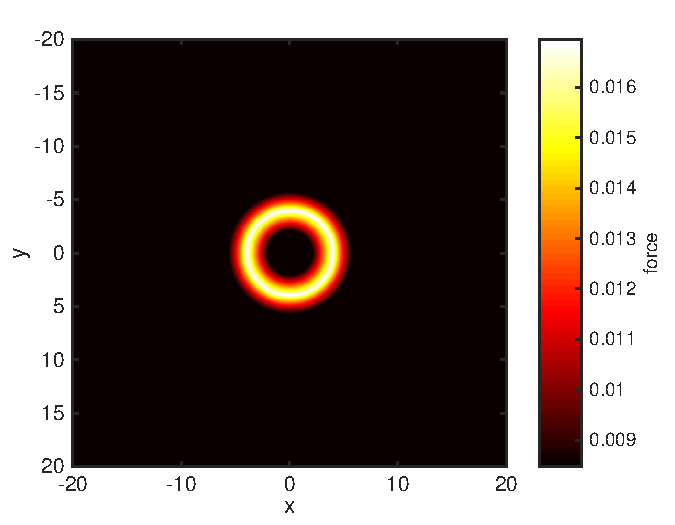
\includegraphics[scale=0.6,angle=0]{images/sp_lorho_force_final.pdf}}
\subfigure[\,  Force as function of distance from   origin ]{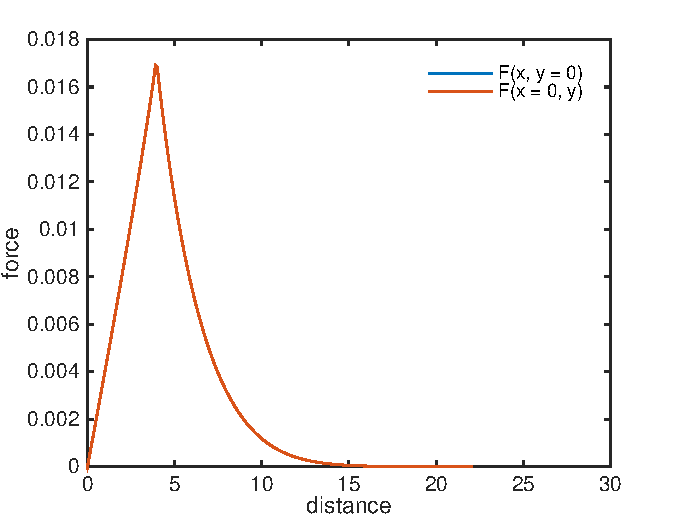
\includegraphics[scale=0.6,angle=0]{images/sp_lorho_fxy_force_final.pdf}}
      \end{center}
\caption{ The force due to the chameleon around a circular source. This source has size $R=4$. The other parameter values are those given in (\ref{paramvalues}).  Note that the force increases linearly from the origin, until some maximum is reached at the objects surface: the force then decreases as $r^{-2}$. \note{replace with converged versions}}\label{fig:circ}
\end{figure}

\subsection{Ellipsoidal sources}
Here we define the shape to be inside the ellipse
\bea
\label{ellipse-eq}
\left( \frac{x}{b}\right)^2 + \left( \frac{y}{a}\right)^2 = R^2
\eea
See \fref{fig:ellip}.
\begin{figure}[!t]
      \begin{center}
\subfigure[\, Force density (2D) ]{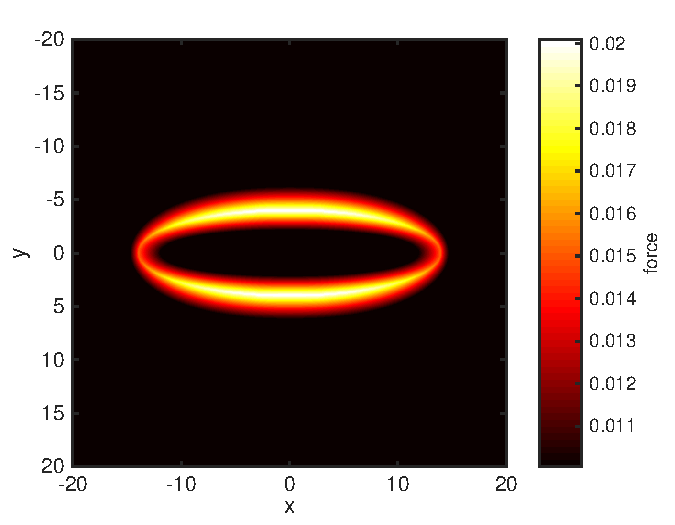
\includegraphics[scale=0.6,angle=0]{images/el_lorho_force_final.pdf}}
\subfigure[\, Force as function of distance from   origin ]{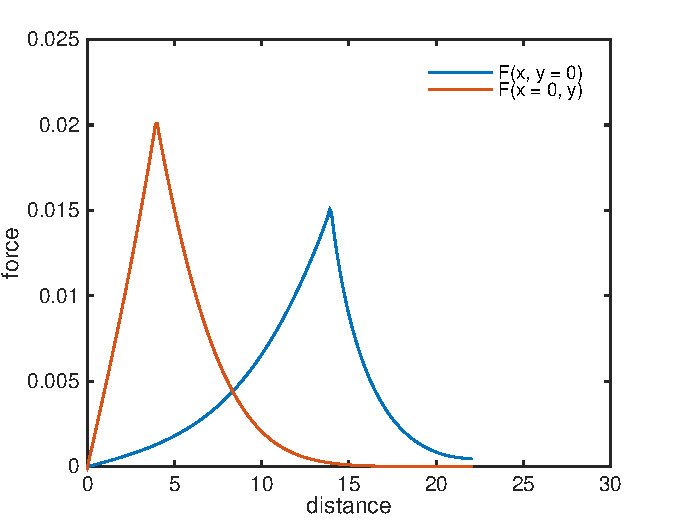
\includegraphics[scale=0.6,angle=0]{images/el_lorho_fxy_force_final.pdf}}
      \end{center}
\caption{ Force due to the chameleon around an ellipsoidal source. This source  has $a = 3.5, b = 1$, and $R=4$ as defined in (\ref{ellipse-eq}); the densities and all other parameters are the same as the source shown in \fref{fig:circ}. Here we observe that the force profiles along the $x$- and $y$-axes are rather different. The force at the object's surface at $y=0$ is lower than the force at the object's surface at $x=0$. Additionally, the force profile inside the object is markedly different along the two axes: along the $y$-axis the force profile is approximately linear, but along the $x$-axis it is parabolic. \note{replace with converged versions} }\label{fig:ellip}
\end{figure}

\subsection{Other shapes}
\fref{fig:varioushapes}.

\begin{figure}[!t]
      \begin{center}
\subfigure[\, Crossed ellipses ]{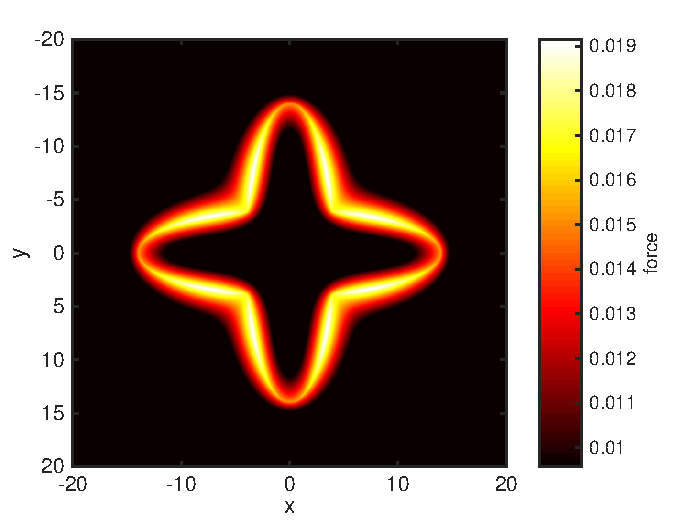
\includegraphics[scale=0.6,angle=0]{images/ep2_lorho_force_final.pdf}}
      \end{center}
\caption{ The force due to the chameleon around various sources. In (a) there are two ellipses at right-angles each with the same properties as those in \fref{fig:ellip}.  \note{replace with converged versions}}\label{fig:varioushapes}
\end{figure}

\section{Using the \textit{cartoon} method to shape chameleons in 3D}
Our codes use gradient flow to obtain the shape of the chameleon fields in 2D. This is an initial choice, born out of numerical simplicity (as well as being able to easily see everything that is going on). However, as discussed in Appendix \ref{poissonseqsoln}, the gravitational potential in 2D and 3D are rather different in nature: and so we want to be able to test whether force discrepancies in 2D are due to the chameleon, or because we are using 2D. 

It is now to be remarked that whilst the numerical algorithms are simple to extend from 2D to 3D, the increase in computational resources is substantial. And so, we assume that the source in 3D is cylindrically symmetric, which allows us to obtain the chameleon profiles in a 2D slice of the object: this slice must be rotated forwards and backwards to capture the 3D-ness. One can also impose some periodic breaking of cylindrical symmetry. This is the essence of the \textit{cartoon} method. 

The idea is to perform gradient flow in Cartesian coordinates in the $(x,y,z) = (x,0,z)$-plane, and then extrapolate the fields into the $y = \pm \Delta x$ planes using the assumed cylindrical symmetry. This strategy has been sucessfully used in the construction of cylindrically symmetric solitons, specifically cosmic vortons (of both global and gauged kind).

\section{Discussion}

\addcontentsline{toc}{section}{Acknowledgements}

\section*{Acknowledgements}

\appendix
\section{Numerical methods}
\label{sec:nummethods}
In summary, our numerical methodology is:
\begin{itemize}
\item Solve for the chameleon scalar (\ref{eq:cham-eom}) via gradient flow; finite difference derivatives discretized to fourth order accuracy.
\item Solve Poisson's equation (\ref{eq:laplaceseqn}) via SoR; discretized to second order accuracy.
\item The forces (\ref{eq:forces}) are computed with finite difference derivatives discretized to fourth order
\end{itemize}
In the remainder of this Appendix we shall explain the implementation of each of these methods.

\subsection{Gradient flow}
The scalar field profile is obtained by solving the gradient flow equation:
\bea
\label{gfeqn}
\dot{\phi} = \nabla^2\phi - \frac{\dd\qsubrm{V}{eff}}{\dd\phi}.
\eea
We discretize the time derivative in a very simple manner,
\bea
\dot{\phi} \approx \frac{\phi(t+1) - \phi(t)}{h_t}.
\eea
This can be used on the LHS of (\ref{gfeqn}) to yield an updating algorithm for the scalar; obviously, we also need a scheme to approximate the Laplacian: that is discussed in the next section. Note that we use a ``fictitious time-step'', $h_t$: this must be chosen to be much smaller than any  step-sizes in the spatial dimensions (else the problem is badly defined numerically).

A ``solution'' to the static problem is obtained when $\dot{\phi}=0$. This is quantified by computing an error estimate
\bea
E_{\phi} \defn \int \dd^2x\, \dot{\phi},
\eea
and waiting until $E_{\phi}\ll \varepsilon$, where $\epsilon$ is supposed to be a very small number, before a solution is declared to have been found. We are also estimating the error on a solution by computing the evolution of the integral of the modulus of the force,
\bea
\qsuprm{E}{F}_{\phi} \defn \int \dd^2x\, \left| \rbm{F}_{(\phi)}\right|;
\eea
this quantity should be independant of time, and so we wait until $\dot{E}\qsuprm{}{F}_{\phi}\ll \varepsilon$ before declaring that a solution has been found.



\subsection{Discretization schemes}
Here we explain the discretization schemes used. Space is discretized onto a lattice with step-size $h$.

\subsubsection{Fourth order finite difference derivatives}
The first and second derivatives of a quantity $Q$, say, are approximated at a given location via a fourth-order accurate finite difference scheme according to
\bea
\pd{Q}{x} \approx \frac{-Q_{i+2} + 8 Q_{i+1} - 8 Q_{i-1} + Q_{i-2}}{12h},
\eea
\bea
\pd{^2Q}{x^2} \approx \frac{-Q_{i+2} + 16 Q_{i+1} - 30 Q_i + 16 Q_{i-1} - Q_{i-2}}{12h^2}.
\eea
There are obvious equivalents for the $y$-derivatives.

\subsubsection{SoR} 
This is used to solve Laplace's equation. Fictitious ``time-steps'' are used, and indexed by $n$. Convergence is determined by the parameter $\omega$. The updating algorithm is
\bea
Q^{n+1}_{i,j} = (1-\omega) Q^{n}_{i,j} + \frac{\omega}{4}\left[ Q^n_{i+1,j} + Q^{n+1}_{i-1,j} + Q^n_{i,j+1} + Q^{n+1}_{i,j-1} + h^2\rho \right]
\eea

\subsection{Simulated annealing}
We have a suggestion to obtain the optimal shape via simulated annealing. This would be implemented by first specifying some given matter distribution (e.g., a sphere), and computing the scalar and gravitational forces. A new shape is randomly proposed -- by switching ``on'' or ``off'' locations which are supposed to have matter. If the force discrepancies are greater for this new shape, it is kept, and the whole process is repeated until an optimal shape is obtained. One needs to be careful to only proposed connected objects.

This strategy is relatively straight-forward, but computationally very intensive -- one way to help is to parallelise the code.
\section{Solving Poisson's equation for symmetric sources}
\label{poissonseqsoln}
Here we solve Poisson's equation, 
\bea
\nabla^2\Phi = - \rho /M,
\eea
for a source with constant density $\rho_0$ immersed in a medium with density $\qsubrm{\rho}{bg}$; the source has radius $R$.
\subsection{Poisson's equation in 2D}
Here we assume a 2D  circular source. Due to the symmetry of the source, the gravitational potential $\Phi = \Phi(r)$ only. Note that the Laplacian in 2D polars is
\bea
\nabla^2\Phi = \frac{1}{r}\frac{\dd}{\dd r}\left( r \frac{\dd\Phi}{\dd r}\right).
\eea
The solution is
\bea
\Phi(r) = -\frac{\rho}{4M}r^2 + A\ln r + B,
\eea
where $A$ and $B$ are integration constants; their values will be fixed by requiring continuity, smoothness, and regularity in various regimes. The radial component of the force (the only component, infact) is
\bea
F_r(r) =  \frac{\rho}{2M}r - \frac{A}{r}.
\eea
From hereon we will drop the ``$r$'' index from the force component.
We are interested in obtaining the gravitational potential surrounding and within a circle of radius $R$, density $\rho_0$, immersed in a background density $\qsubrm{\rho}{bg}$. One requires $\qsubrm{A}{in}=0$ for regularity at the origin. By matching the forces at the surface $r=R$ one obtains the   expression for $\qsubrm{A}{out}$,
\bse
\bea
\qsubrm{A}{out} = \frac{ \qsubrm{\rho}{bg}R^2}{2M}\left( 1 - \frac{\rho_0}{\qsubrm{\rho}{bg}}\right).
\eea
By matching the potentials, one also obtains
\bea
\qsubrm{B}{bg} = B_0 + \frac{R^2\qsubrm{\rho}{bg}}{4M}\left( 1- \frac{\rho_0}{\qsubrm{\rho}{bg}}\right)\left( 1 - 2\ln R\right).
\eea
\ese


The potential inside and outside the object is given by
\bse
\label{poiss-soln-1}
\bea
\qsubrm{\Phi}{in}(r) = - \frac{\rho_0}{4M}r^2 + B_0,
\eea
\bea
\qsubrm{\Phi}{out}(r) = - \frac{\qsubrm{\rho}{bg}}{4M}r^2 +  \frac{ \qsubrm{\rho}{bg}R^2}{2M}\left( 1 - \tfrac{\rho_0}{\qsubrm{\rho}{bg}}\right)\ln r + B_0+ \frac{R^2\qsubrm{\rho}{bg}}{4M}\left( 1- \tfrac{\rho_0}{\qsubrm{\rho}{bg}}\right)\left( 1 - 2\ln R\right),\nonumber\\
\eea
\ese
and the force inside and outside are given by
\bse
\label{poiss-soln-2}
\bea
\qsubrm{F}{in}(r) = \frac{\rho_0}{2M}r,
\eea
\bea
\qsubrm{F}{out}(r) =  \frac{\qsubrm{\rho}{bg}}{2M}r -   \frac{\qsubrm{\rho}{bg}R^2}{2M}{}{ }\left( 1 -\tfrac{ \rho_0}{\qsubrm{\rho}{bg}} \right) \frac{1}{r} .
\eea
\ese
See \fref{fig:poisson_soln} for a plot of these solutions.
\subsection{Poisson's equation in 3D}
In 3D, for a spherically symmetric gravitational potential, the Laplacian reads
\bea
\nabla^2\Phi = \frac{1}{r^2}\frac{\dd}{\dd r}\left( r^2 \frac{\dd\Phi}{\dd r}\right).
\eea
The solution to Poisson's equation (again, with a constant source density $\rho$) is 
\bea
\Phi(r) = - \frac{\rho}{6M} r^2- \frac{A}{r}+ B,
\eea
in terms of two integration constants $A$ and $B$.   After requiring  continuity and regularity, the potential and force inside and out are given by
\bse
\label{poiss-soln-3}
\bea
\qsubrm{\Phi}{in}(r) = - \frac{\qsubrm{\rho}{in}}{6M} r^2 + \qsubrm{B}{in},
\eea
\bea
\qsubrm{\Phi}{out}(r) = - \frac{\qsubrm{\rho}{out}}{6M} r^2+ \frac{\qsubrm{\rho}{out}R^3}{3M} \left(\tfrac{\qsubrm{\rho}{in} }{\qsubrm{\rho}{out}} -1\right) \frac{1}{r}+\frac{\qsubrm{\rho}{out}R^2}{2M} \left(1 - \tfrac{\qsubrm{\rho}{in}}{\qsubrm{\rho}{out}}\right)  +\qsubrm{B}{in},
\eea
\ese
\bse
\label{poiss-soln-4}
\bea
\qsubrm{F}{in} (r)=  \frac{\qsubrm{\rho}{in}}{3M} r,
\eea
\bea
\qsubrm{F}{out}(r) = \frac{\qsubrm{\rho}{out}}{3M} r+\frac{\qsubrm{\rho}{out}R^3}{3M} \left(\tfrac{\qsubrm{\rho}{in} }{\qsubrm{\rho}{out}}-1 \right)  \frac{1}{r^2} .
\eea
\ese
See \fref{fig:poisson_soln} for a plot of these solutions.

\begin{figure}[!t]
      \begin{center}
{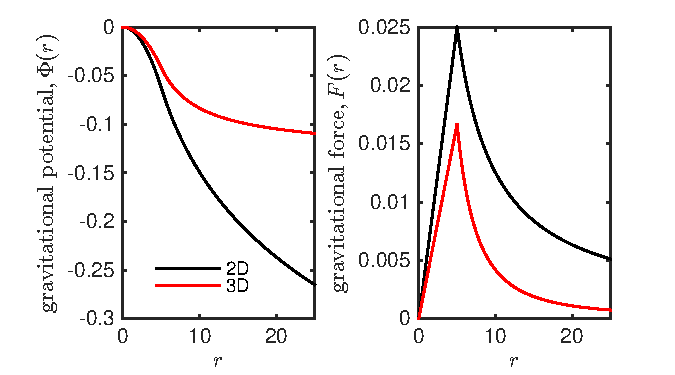
\includegraphics[scale=1.4,angle=0]{images/rhoin_10_comps}}
      \end{center}
\caption{ The gravitational potential (left) and force (right) for 2D and 3D circularly and spherically symmetric sources with constant density. These correspond to the solutions we presented in (\ref{poiss-soln-1},  \ref{poiss-soln-2},  \ref{poiss-soln-3},  \ref{poiss-soln-4}). }\label{fig:poisson_soln}
\end{figure}

\addcontentsline{toc}{section}{References}
\bibliographystyle{JHEP}
\footnotesize{
\bibliography{refs}
}
\end{document}
